% Fig. 1 of the manuscript: overview of the transformation (compiled to figures/fig_overview.pdf by make_schematics.py)
\documentclass[border=1pt]{standalone}
\usepackage[T1]{fontenc}
\usepackage[scaled]{helvet}
\renewcommand{\familydefault}{\sfdefault}
\usepackage{courier}
\usepackage{amsmath}
\usepackage{sansmath}
\sansmath
\usepackage{tikz}
\usetikzlibrary{positioning,arrows.meta,calc,fit,backgrounds,shapes.misc}

% plain style of the flowcharts in APL Computational Physics: black outlines, grey panels, sans-serif text
\definecolor{ink}{HTML}{000000}
\definecolor{muted}{HTML}{555555}
\definecolor{rule}{HTML}{000000}
\definecolor{cI}{HTML}{1F77B4}
\definecolor{cII}{HTML}{FF7F0E}
\definecolor{cIII}{HTML}{2CA02C}
\definecolor{bad}{HTML}{D62728}
\definecolor{code}{HTML}{000000}
\definecolor{kw}{HTML}{1F77B4}
\definecolor{hl}{HTML}{FFFFFF}

\tikzset{
  >={Stealth[length=5pt,width=4pt]},
  every node/.style={text=ink, font=\footnotesize},
  card/.style={draw=black, fill=black!10, rounded corners=2pt, line width=0.6pt},
  head/.style={fill=black!65, rounded corners=2pt, text=white, font=\footnotesize\bfseries, inner sep=3.2pt},
  chip/.style={draw=black, fill=white, rounded corners=2pt, inner xsep=5pt, inner ysep=3pt, font=\scriptsize,
    minimum width=3.25cm, align=center, line width=0.5pt},
  lane/.style={rounded corners=2pt, line width=0.6pt},
  badge/.style={circle, inner sep=0pt, minimum size=0.58cm, text=white, font=\footnotesize\bfseries,
    draw=black, line width=0.5pt},
  cell/.style={align=center, font=\scriptsize, inner sep=1pt},
  flow/.style={->, line width=0.8pt, draw=black},
  lbl/.style={font=\scriptsize\itshape, text=muted},
  tag/.style={font=\footnotesize\bfseries, text=ink, anchor=west},
  it/.style={draw=black, fill=white, rounded corners=1pt, minimum width=0.62cm, minimum height=0.46cm,
    font=\scriptsize, inner sep=0pt, line width=0.5pt},
  tape/.style={draw=black, fill=black!35, minimum width=0.62cm, minimum height=0.13cm, inner sep=0pt,
    line width=0.4pt},
  codefont/.style={font=\ttfamily\fontsize{6.6}{8.5}\selectfont, text=code},
}
\newcommand{\kw}[1]{\textcolor{kw}{\textbf{#1}}}

\begin{document}
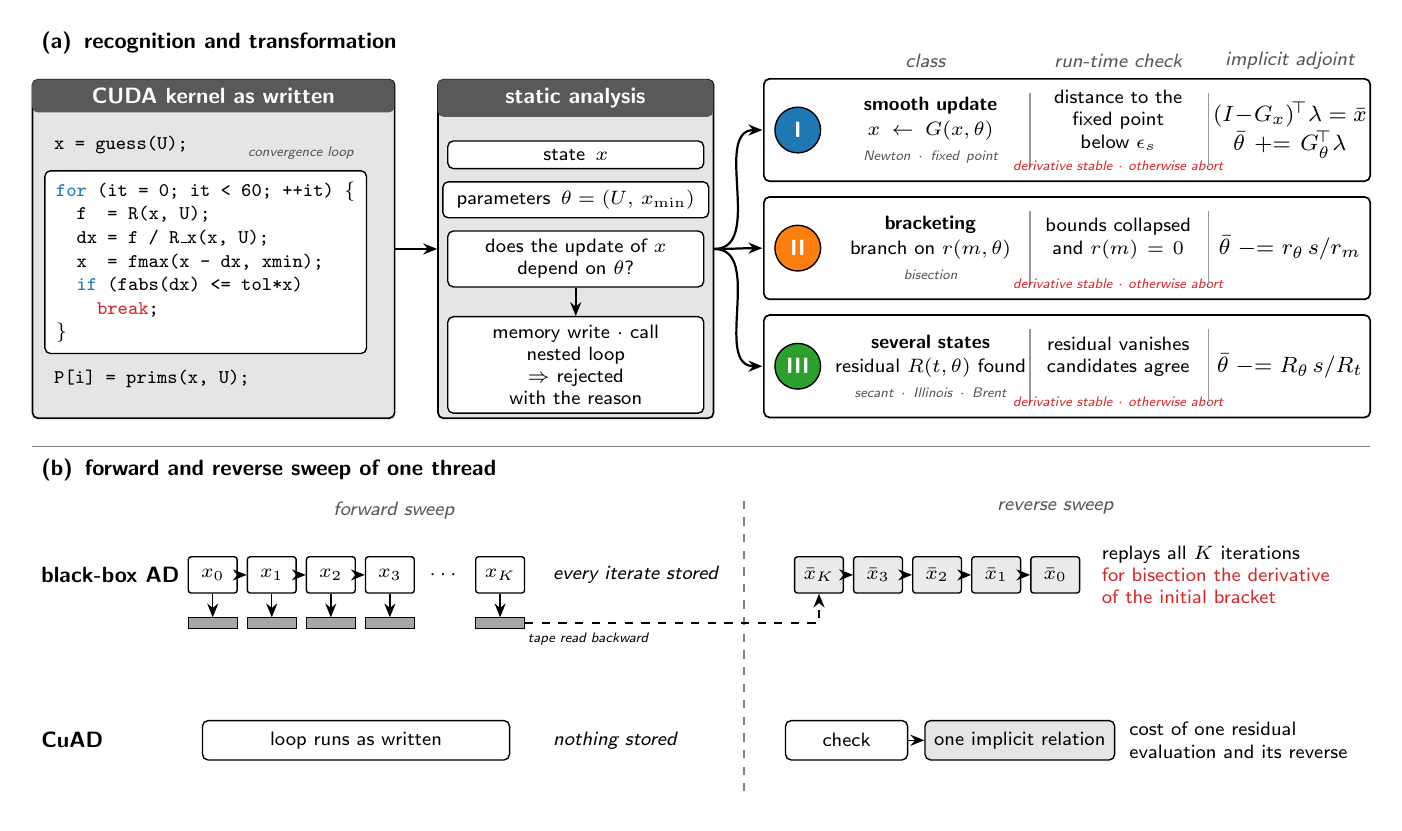
\begin{tikzpicture}[x=1cm, y=1cm]
\useasboundingbox (-0.05,0.55) rectangle (17.05,10.4);

% ---------------------------------------------------------------- (a) pipeline
\node[tag] at (0,10.2) {(a)\enspace recognition and transformation};

% code card
\node[card, minimum width=4.6cm, minimum height=4.3cm, anchor=north west] (code) at (0,9.75) {};
\node[head, anchor=north west, minimum width=4.6cm] at (code.north west) {CUDA kernel as written};
\node[anchor=north west, codefont, inner sep=0pt] (c1) at ($(code.north west)+(0.28,-0.72)$) {x = guess(U);};
\node[anchor=north west, fill=white, draw=black, rounded corners=2pt, line width=0.5pt, inner xsep=4pt, inner ysep=4pt, codefont,
  align=left] (loop) at ($(c1.south west)+(-0.12,-0.2)$) {%
\kw{for} (it = 0; it < 60; ++it) \{\\
\ \ f\ \ = R(x, U);\\
\ \ dx = f / R\_x(x, U);\\
\ \ x\ \ = fmax(x - dx, xmin);\\
\ \ \kw{if} (fabs(dx) <= tol*x)\\
\ \ \ \ \textcolor{bad}{\textbf{break}};\\
\}};
\node[anchor=north west, codefont, inner sep=0pt] (c3) at ($(loop.south west)+(0.12,-0.2)$) {P[i] = prims(x, U);};
\node[lbl, anchor=south east, font=\tiny\itshape] at ($(loop.north east)+(-0.05,0.02)$) {convergence loop};

% analysis card
\node[card, minimum width=3.5cm, minimum height=4.3cm, anchor=north west] (ana) at (5.15,9.75) {};
\node[head, anchor=north west, minimum width=3.5cm] at (ana.north west) {static analysis};
\node[chip, anchor=north] (k1) at ($(ana.north)+(0,-0.78)$) {state\enspace $x$};
\node[chip, below=0.15cm of k1] (k2) {parameters\enspace $\theta=(U,\,x_{\min})$};
\node[chip, below=0.15cm of k2] (k3) {does the update of $x$\\ depend on $\theta$?};
\node[chip, draw=black, fill=white, below=0.36cm of k3, text width=2.9cm] (rej)
  {memory write $\cdot$ call\\ nested loop\\ $\Rightarrow$ rejected with the reason};
\draw[flow] (code.east) -- (ana.west);
\draw[->, line width=0.6pt, draw=black] (k3.south) -- (rej.north);

% three lanes: class | run-time check | implicit adjoint
\def\lx{9.3} \def\lw{7.7}
\foreach \y/\c/\n/\title/\rel/\ex/\chk/\adj in {
  9.1/cI/I/smooth update/{$x\leftarrow G(x,\theta)$}/{Newton $\cdot$ fixed point}/{distance to the\\ fixed point below $\epsilon_s$}/{$(I-G_x)^{\!\top}\lambda=\bar x$\\[1pt] $\bar\theta\mathrel{+}=G_\theta^{\!\top}\lambda$},
  7.6/cII/II/bracketing/{branch on $r(m,\theta)$}/{bisection}/{bounds collapsed\\ and $r(m)=0$}/{$\bar\theta\mathrel{-}=r_\theta\,s/r_m$},
  6.1/cIII/III/several states/{residual $R(t,\theta)$ found}/{secant $\cdot$ Illinois $\cdot$ Brent}/{residual vanishes\\ candidates agree}/{$\bar\theta\mathrel{-}=R_\theta\,s/R_t$}} {
  \draw[lane, draw=black, fill=white] (\lx,\y-0.65) rectangle ++(\lw,1.3);
  \node[badge, fill=\c] at (\lx+0.43,\y) {\n};
  \node[cell, anchor=west, text width=2.45cm] at (\lx+0.85,\y)
    {\textbf{\title}\\[1pt] \rel\\[1pt] {\color{muted}\itshape\tiny \ex}};
  \draw[line width=0.5pt, draw=black!40] (\lx+3.38,\y-0.47) -- (\lx+3.38,\y+0.47);
  \node[cell, anchor=center, text width=2.1cm] at (\lx+4.5,\y+0.12) {\chk};
  \node[cell, anchor=center, text=bad, font=\tiny\itshape] at (\lx+4.5,\y-0.45) {derivative stable $\cdot$ otherwise abort};
  \draw[line width=0.5pt, draw=black!40] (\lx+5.65,\y-0.47) -- (\lx+5.65,\y+0.47);
  \node[cell, anchor=center, text width=1.95cm, font=\footnotesize] at (\lx+6.68,\y) {\adj};
  \draw[flow] (ana.east) to[out=0, in=180] (\lx-0.02,\y);
}
\node[lbl] at (\lx+2.05,9.98) {class};
\node[lbl] at (\lx+4.5,9.98) {run-time check};
\node[lbl] at (\lx+6.68,9.98) {implicit adjoint};

% ---------------------------------------------------------------- (b) sweeps
\draw[black!50, line width=0.5pt] (0,5.08) -- (17,5.08);
\node[tag] at (0,4.78) {(b)\enspace forward and reverse sweep of one thread};
\draw[dashed, black!50, line width=0.6pt] (9.05,0.7) -- (9.05,4.4);
\node[lbl, anchor=north] at (4.6,4.5) {forward sweep};
\node[lbl, anchor=north] at (13.0,4.5) {reverse sweep};

% program AD
\node[font=\footnotesize\bfseries, anchor=west] at (0,3.45) {black-box AD};
\foreach \i/\x in {0/2.3,1/3.05,2/3.8,3/4.55} {
  \node[it] (f\i) at (\x,3.45) {$x_\i$};
  \node[tape, below=0.3cm of f\i] (t\i) {};
  \draw[->, line width=0.5pt, draw=black] (f\i.south) -- (t\i.north);
}
\node[font=\scriptsize] at (5.25,3.45) {$\cdots$};
\node[it] (fK) at (5.95,3.45) {$x_K$};
\node[tape, below=0.3cm of fK] (tK) {};
\draw[->, line width=0.5pt, draw=black] (fK.south) -- (tK.north);
\foreach \a/\b in {f0/f1,f1/f2,f2/f3} \draw[->, line width=0.5pt] (\a) -- (\b);
\node[lbl, anchor=west, text=black] at (6.5,3.45) {every iterate stored};
\foreach \i/\x in {K/10.0,3/10.75,2/11.5,1/12.25,0/13.0} \node[it, fill=black!8] (r\i) at (\x,3.45) {$\bar x_\i$};
\foreach \a/\b in {rK/r3,r3/r2,r2/r1,r1/r0} \draw[->, line width=0.5pt] (\a) -- (\b);
\draw[->, dashed, line width=0.6pt, draw=black] (tK.east) -- ++(1.6,0) node[pos=0.5, below, lbl, font=\tiny\itshape, text=black] {tape read backward}
  -| (rK.south);
\node[cell, anchor=west, text width=3.35cm, align=left] at (13.55,3.45)
  {replays all $K$ iterations\\ {\color{bad}for bisection the derivative\\ of the initial bracket}};

% CuAD
\node[font=\footnotesize\bfseries, anchor=west] at (0,1.35) {CuAD};
\node[draw=black, fill=white, rounded corners=2pt, line width=0.5pt, minimum width=3.9cm, minimum height=0.5cm, font=\scriptsize]
  (fc) at (4.12,1.35) {loop runs as written};
\node[lbl, anchor=west, text=black] at (6.5,1.35) {nothing stored};
\node[draw=black, fill=white, rounded corners=2pt, line width=0.5pt, minimum height=0.5cm, minimum width=1.55cm, font=\scriptsize]
  (rc) at (10.35,1.35) {check};
\node[draw=black, fill=black!10, rounded corners=2pt, line width=0.5pt, minimum height=0.5cm, minimum width=2.25cm, font=\scriptsize]
  (ra) at (12.55,1.35) {one implicit relation};
\draw[->, line width=0.5pt] (rc) -- (ra);
\node[cell, anchor=west, text width=3.35cm, align=left] at (13.9,1.35) {cost of one residual\\ evaluation and its reverse};
\end{tikzpicture}
\end{document}
